La fin d'un projet ne signifie pas que l'application est termin�e, si l'on veut que celle-ci vive il faut toujours l'am�liorer. En ce qui concerne la n�tre, les am�liorations suivantes devraient �tre envisag�e.

\paragraph{L'API de Twitter}
Dans un premier temps, prendre un compte Entreprise qui permet une plus grande libert� pour les d�veloppeurs, lorsque ceci sera fait, il est bien probable qu'il faille �galement changer la r�cup�rations des Tweets. 

\paragraph{L'Optimisations}
Il est toujours possibles d'optimiser un projet d'une mani�re ou d'une autre et le notre n'y fait pas exception, si l'on applique les pr�c�dent points et tout particuli�rement le premier, � savoir un changement d'API, nous aurons un volume de donn�es bien plus important, chaque seconde compte surtout sur le web ou une dizaine de seconde ressemble � une �ternit�. Ajouter Apache Spark, un framework open source de calcul distribu�,au projet serait d�j� un bon point dans ce sens.

\paragraph{Est-ce que l'on viole la vie priv�e des employ�s ?}
Lors de ce projet nous nous sommes surtout pos� la question de savoir si l'on pouvait faire certaine chose avec l'API de Twitter au lieu de nous demander si l'on y avait le droit. Nous sommes parti du principe que Twitter ainsi que les Tweets qui sont dessus font partie du domaine publique. Mais est-ce r�ellement le cas ?

\newpage
\paragraph{L'authentification}
Comme nous avons pu le voir auparavant, notre syst�me d'authentification n'est pas encore au point. L'id�al serait de le r�parer ou m�me de le remplacer. En regardant les recommandation d'OWASP, on voit un framework qui se d�gage du lot, \textbf{lift}. Bien �videmment, �ela signifie qu'il faudrait abandonner Scala-Play et donc il faut bien mesurer les pour et les contres d'un tel changement et mesurer le temps n�cessaire pour le faire.

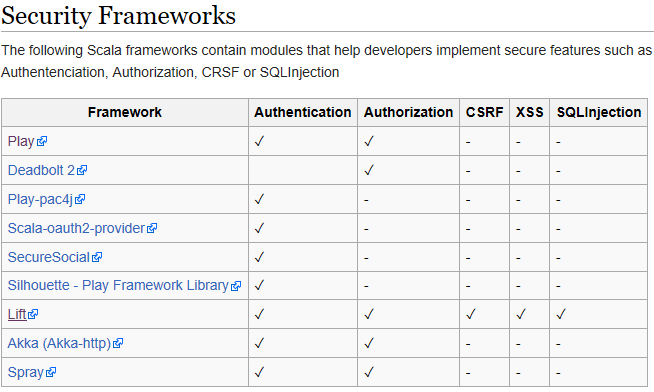
\includegraphics[width=\textwidth]{frameworks}